## Recursividad: Series {.fragile}

\bgnblockgood
\strongText{Ejemplo 6:} Determine la suma de: $1 + 2 + 3 + 4 + \ldots + n$.
\trmblockgood

\pause

\begin{lstlisting}[style=frame02]
# suma1n: int -> int
# Calcula la suma de los primeros n números naturales.
# Ejemplo: suma1n(3) retorna 6
def suma1n(n):
    if n == 1:
        return 1
    else:
        return n + suma1n(n - 1)
# Tests
assert suma1n(1) == 1
assert suma1n(6) == 21
\end{lstlisting}

## Recursividad: Series {.fragile}

\bgnblockgood
\strongText{Ejemplo 7:} Calcule el valor de: $\quad\sum\limits_{0}^n \frac{1}{2^n}$
\trmblockgood

\pause

\begin{small}
\begin{lstlisting}[style=frame02]
# unMedioCeroN: int -> num
# Calcula el valor de la serie cuyo término enésimo es 1/(2^n),
# partiendo desde 0.
# Ejemplo: unMedioCeroN(5) retorna 1.96875
def unMedioCeroN(n):
    if n == 0:
        return 1
    else:
        return (1 / (2.0**n)) + unMedioCeroN(n - 1)
# Tests
assert unMedioCeroN(1) == 1.5
assert unMedioCeroN(6) == 1.984375
\end{lstlisting}
\end{small}

## Recursividad: Series {.fragile}

\bgnblockgood
\strongText{Ejemplo 8:} Calcule el valor de: $\quad\sum\limits_{1}^n \frac{1}{2^n}$
\trmblockgood

\pause

\begin{small}
\begin{lstlisting}[style=frame02]
# unMedioUnoN: int -> num
# Calcula el valor de la serie
# cuyo término enésimo es 1/(2^n),
# partiendo desde 1.
# Ejemplo: unMedioUnoN(5) retorna 0.96875
def unMedioUnoN(n):
    if n == 1:
        return 1/2.0(*@\tikzmark{markBgnHalf}@*)
    else:
        return (1 / (2.0**n)) + unMedioUnoN(n - 1)
# Tests
assert unMedioUnoN(1) == 0.5
assert unMedioUnoN(6) == 0.984375
\end{lstlisting}
\end{small}

\drawTikZComment[pos={above right},len={-0.2em and 7em}, text width=10em]{markBgnHalf}{\scriptsize Ojo, acá el primer valor es $\mathbf{\frac{1}{2}}$}

## Recursividad: Torres de Hanói {.fragile}

- Es un puzzle/juego matemático.
- Consiste en varios discos de distinto tamaño y tres torres.
- La idea es que todos los discos, que inicialmente están en la torre
izquierda, hay que moverlos hasta la torre derecha, respetando las siguientes reglas:
    1. Sólo un disco puede ser movido cada vez.
    1. Un disco sólo puede ser movido sobre una torre vacía o sobre otro disco más grande.

\centering    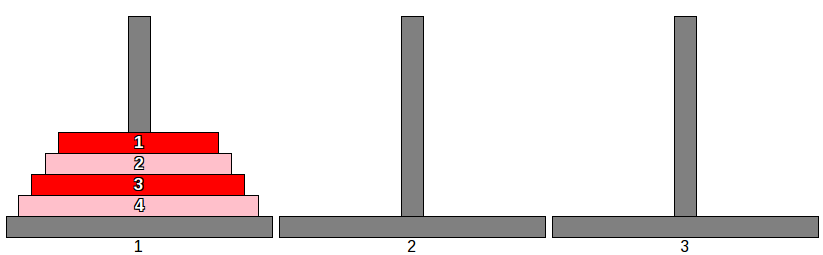
\includegraphics[width=.8\textwidth]{img/towersHanoi.png}

## Recursividad: Torres de Hanói {.fragile}

- Nuestro objetivo es saber cuántos son los pasos mínimos para resolver el juego, dados
$n$ discos.
- También se quiere determinar la mejor secuencia de pasos para resolverlo.

- Se puede ver una demostración interactiva en: \url{https://nozimica.github.io/hanoi/}

## Repaso: recursividad y estimación de PI {.fragile}

\bgnenviron{<1-2>}{onlyenv}

- Todos sabemos que la constante $\pi$ es un número irracional, y por lo tanto, infinito.

\begin{center}
\textsf{$\pi$ = 3,14159265358979323846264338327950288419716939$\ldots$}
\end{center}

\trmenviron{onlyenv}

\bgnenviron{<2-3>}{onlyenv}

- Pero existe la llamada ``serie de Leibniz'' con la cual se puede calcular un valor aproximado de $\pi$:

\vspace{-3ex}
$$ \frac{\pi}{4} = \left( 1 - \frac{1}{3} + \frac{1}{5} - \frac{1}{7} + \frac{1}{9} - \frac{1}{11} + \ldots + \frac{(-1)^{n}}{2n + 1} \right) = \sum_{n=0}^{N} \frac{(-1)^{n}}{2n + 1} $$

\trmenviron{onlyenv}

\bgnenviron{<2>}{onlyenv}

- Mientras más grande sea $N$, más cerca estaremos del valor ``verdadero'' de $\pi$.

\trmenviron{onlyenv}

\bgnenviron{<3-6>}{onlyenv}

\simpleTitle{Solución recursiva:}

- \bld{Caso base:}
    - $n = 0$
    - Resultado: $1$
- \bld{Caso recursivo:} Retorno la suma de:
    - El n-ésimo valor de la serie.\tikzmark{markNthValueText}
    - La función reducida a $n \tikzmark{markRecCallText}- 1$.

\trmenviron{onlyenv}

\bgnenviron{<5-6>}{onlyenv}

\vspace{2ex}

\begin{lstlisting}[style=frame02]
def calcPI(n):
    return 4 * seriePI4(n)

def seriePI4(n):
    if n == 0:
        return 1
    else:
        return (*@\tikzmark{markBgnNthValue}@*)(-1)**(n) / (2*n + 1.0)(*@\tikzmark{markTrmNthValue}@*) + (*@\tikzmark{markBgnRecCall}@*)seriePI4(n - 1)(*@\tikzmark{markTrmRecCall}@*)
\end{lstlisting}

\trmenviron{onlyenv}

\bgnenviron{<6>}{onlyenv}

\braceUpwards[decoration/.style={decoration={brace,raise=0pt,amplitude=0.5em},decorate,ultra thick,structure!80,font=\footnotesize}]{markBgnNthValue}{markTrmNthValue}
\braceUpwards[decoration/.style={decoration={brace,raise=0pt,amplitude=0.5em},decorate,ultra thick,structure!80,font=\footnotesize}]{markBgnRecCall}{markTrmRecCall}

\begin{tikzpicture}[remember picture, overlay]
    \draw[thick, structure!80,->,-Stealth] ([shift={(0,.5ex)}]pic cs:markNthValueText) to[out=0,in=90] ($(markBgnNthValuemarkTrmNthValue)+(0,5mm)$);
    \draw[thick, structure!80,->,-Stealth] (pic cs:markRecCallText) to[out=-90,in=90] ($(markBgnRecCallmarkTrmRecCall)+(0,5mm)$);
\end{tikzpicture}

\trmenviron{onlyenv}

## Repaso: recursividad y estimación de PI {.fragile}

\simpleTitle{Observaciones:}

- Esta serie es conocida por ``converger'' muy lentamente.
    - Hay que entregar un $n$ muy alto para que empiecen a aparecer los primeros decimales conocidos.


\bgnblockgood
\bld{Ejercicio propuesto:} Implementa la ``Transformación de Shanks de la Serie de Leibniz'', que es
una serie que converge más rápido:

\vspace{-3ex}
$$ \frac{\pi}{4} = \sum_{i=0}^{N} \left( \frac{1}{4n + 1} - \frac{1}{4n + 3} \right) $$

\trmblockgood

